% !TEX root = main2.tex
\subsection{Experiments on trace containment reasoning}
\label{sec: sub_exp}
%We describe two experiments illustrating applications of the above results. 

\paragraph{Graph simulation}
Consider the $\auto{AEB}$ system of Section~\ref{ssec:adas} with the
scenario where Vehicle B is stopped ahead of vehicle A, and A transits
from \Lmode{cruise} to \Lmode{em\_brake} to avoid colliding with B.
In the actual system ($G_2$ of Figure~\ref{fig: em_brake_graphs}), two different sensor systems
trigger the obstacle detection and emergency braking at time intervals
$[1,2]$ and $[2.5,3.5]$ and take the system from vertex $0$
(\Lmode{cruise}) to two different vertices labeled with
\Lmode{em\_brake}.

\begin{figure}[ht]
    \begin{subfigure}[b]{0.3\textwidth}
        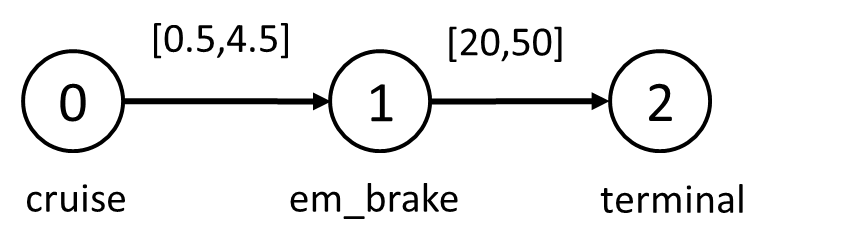
\includegraphics[width=\textwidth]{brake_2_modes.png}
        \caption{\small Transition graph $G_1$.}
        \label{fig: em_brake_graphsA}
    \end{subfigure}
    \begin{subfigure}[b]{0.3\textwidth}
        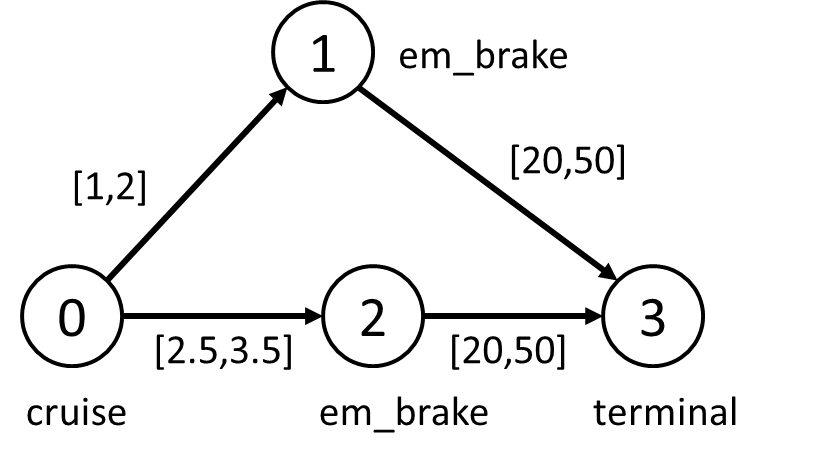
\includegraphics[width=\textwidth]{brake_3_modes.png}
        \caption{Transition graph $G_2$.}
        \label{fig: em_brake_graphsB}
    \end{subfigure}
    \begin{subfigure}[b]{0.35\textwidth}
	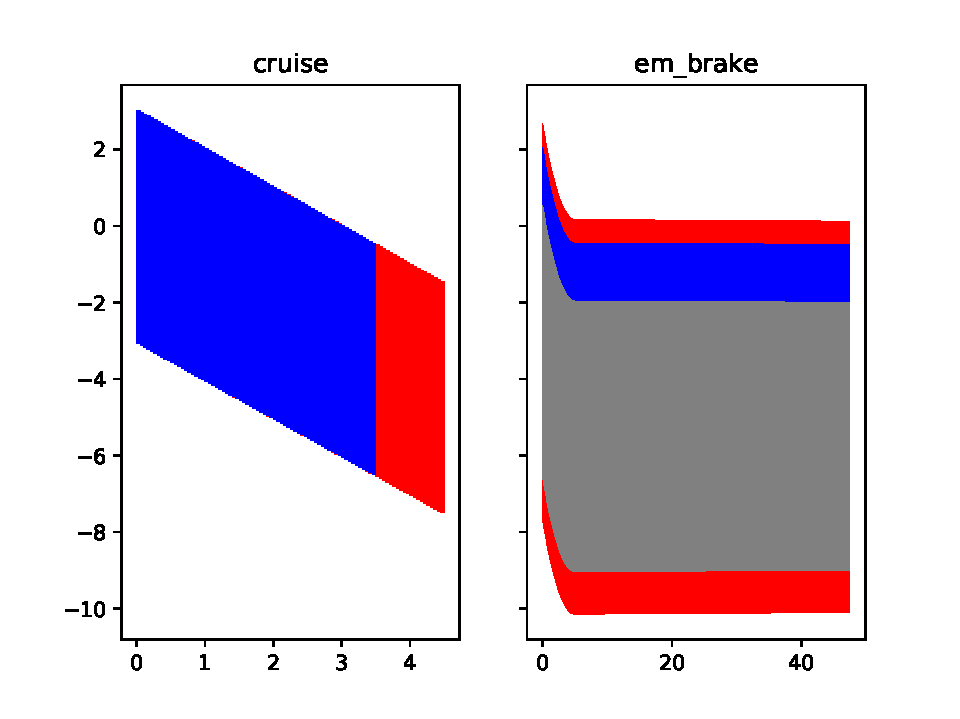
\includegraphics[width=\textwidth]{Abstraction_reachTube.pdf}
	\caption{$\auto{AEB}$ Reachtubes.}
	%\caption{Reachtubes of graphs in Figure \ref{fig: em_brake_graphs}. Red tubes corresponds to Figure \ref{fig: em_brake_graphsA}, blue and gray tubes corresonds to Figure \ref{fig: em_brake_graphsB}}
	\label{fig:abstraction}
    \end{subfigure}
\caption{\small Graphs and reachtubes for the Automatic Emergency Braking $\auto{AEB}$ system.}
\label{fig: em_brake_graphs}
\end{figure}

%
To illustrate trace containment reasoning, consider a simpler
graph $G_1$ that allows a single transition of A from \Lmode{cruise}
to \Lmode{em\_brake} over the interval bigger $[0.5, 4.5]$. Using
Proposition~\ref{prop:hybrid-contain} and checking that graph $G_2
\preceq_{\sf id} G_1$, it follows that verifying the safety of
$\auto{AEB}$ with $G_1$ is adequate to infer the safety with $G_2$.
Figure~\ref{fig:abstraction} shows that the safe reachtubes returned
by the algorithm for $G_1$ in red, indeed contain the reachtubes for
$G_2$ (in blue and gray).
%The graphs of the system, along with the reachtube plots are provided in the Appendix.
%For more complex graphs  

%Figure \ref{fig: em_brake_graphs} shows two different graphs specifying two scenarios.  
%Figure \ref{fig: em_brake_graphsA} shows that vehicle A could transit from \Lmode{cruise} to \Lmode{em\_brack} within $[0.5, 4.5]$. However, in  Figure \ref{fig: em_brake_graphsB} the transition may happen in two disjoint time intervals $[1,2],[2.5,3.5]$. 

%Since both the vehicles never change the lane, we will only consider variables along the $y$ coordinate. The initial set is $sy_A \in [-3,3], sy_B \in [14,23], vy_A = 1, vy_B =0$. The unsafe set is set to be $|sy_A-sy_B| < 2$ ($|sx_A-sx_B| < 2$ is always satisfied).

% In the \Lmode{cruise} mode, the red tube corresponds to the vertex $0$'s reachtube in Figure~\ref{fig: em_brake_graphsA} and the blue one corresponds to vertex $0$ in Figure \ref{fig: em_brake_graphsB}. Similarly, in the \Lmode{em\_brake}, the red tube corresponds to the vertex $0$'s reachtube in Figure \ref{fig: em_brake_graphsA}, the blue tube corresponds to the vertex $1$'s reachtube in Figure \ref{fig: em_brake_graphsB} and the gray tube corresponds to the vertex $2$'s reachtube in Figure \ref{fig: em_brake_graphsB}. It can be clearly seen from Figure \ref{fig:abstraction} that in both modes,  the reachtubes of Figure \ref{fig: em_brake_graphsB} is contained in the reachtube of Figure \ref{fig: em_brake_graphsA}, which is consistent with proposition \ref{prop:hybrid-contain}.


\vspace{-10pt}
\paragraph{Sequential composition}
We revisit the $\auto{Powertrn}$ example of
Section~\ref{ex:powertrain}. The initial set $\Theta$ and unsafe set
are the same as in Table \ref{table:results}.  Let $G_A$ be the graph
($v_0$,\Lmode{startup}) $\xrightarrow{[5,10]}$ ($v_1$,\Lmode{normal})
$\xrightarrow{[10,15]}$ ($v_2$,\Lmode{powerup}), and $G_B$ be the
graph ($v_0$,\Lmode{powerup}) $\xrightarrow{[5,10]}$
($v_1$,\Lmode{normal}) $\xrightarrow{[10,15]}$
($v_2$,\Lmode{powerup}).  The graph $G_1 =$ ($v_0$,\Lmode{startup})
$\xrightarrow{[5,10]}$ ($v_1$,\Lmode{normal}) $\xrightarrow{[10,15]}$
($v_2$,\Lmode{powerup}) $\xrightarrow{[5,10]}$ ($v_3$,\Lmode{normal})
$\xrightarrow{[10,15]}$ ($v_4, $\Lmode{powerup}), can be expressed as
the composition $G_1 = G_A \seqcomp G_B$. Consider the two hybrid
systems $\H_i = \langle \L, \Theta_i, G_i, \TL \rangle$, $i \in
\{A,B\}$ with $\Theta_A = \Theta$ and $\Theta_B =
\reach{\H_A}^{v_2}$. {\toolname}'s estimate of $\Theta_{B}$ had
$\lambda$ in the range from $14.68$ to $14.71$. The reachset
$\reach{\H_B}^{v_2}$ computed by {\toolname} had $\lambda$ from
$14.69$ to $14.70$. The remaining variables also were observed to
satisfy the containment condition. Therefore, $\reach{\H_B}^{v_2}
\subseteq \Theta_{B}$.  Consider the two hybrid systems $\H_i =
\langle \L, \Theta, G_i, \TL \rangle$, $i \in \{1,2\}$, where $G_1$ is
(defined above) $ G_A \seqcomp G_B$, and $G_2 = G_A \seqcomp G_B
\seqcomp G_B \seqcomp G_B$.  Using Theorem
\ref{thm:seqcomp-mainresult} it suffices to analyze $\H_1$ to verify
$\H_2$.  $\H_1$ was been proved to be safe by \toolname\ without any
refinement.  As a sanity check, we also verified the safety of $\H_2$.
%is \Lmode{normal} $\xrightarrow{[10,15]}$ \Lmode{powerup} $\xrightarrow{[5,10]}$ \Lmode{normal} $\xrightarrow{[10,15]}$ \Lmode{term} $\xrightarrow{[0,0]}$ \Lmode{powerup} $\xrightarrow{[5,10]}$ \Lmode{normal} $\xrightarrow{[10,15]}$ %\Lmode{term} $\xrightarrow{[0,0]}$ \Lmode{powerup} $\xrightarrow{[5,10]}$ \Lmode{normal} $\xrightarrow{[10,15]}$ \Lmode{term}. 
{\toolname} proved $\H_2$ safe without any refinement as well.
